%% Cumulative Volcanic Burial and the Archaeological Detection Horizon in Java
%% v5.0 — Provocateur pivot (Session 19 late, 2026-04-21)
%%
%% v4.0 -> v5.0 changes driven by:
%%   (a) 5-model convergent critical review (DeepSeek + Gemini Flash + user's Gemini/ChatGPT/GLM)
%%   (b) Return to original v0.1 (Feb 2026) modest framing
%%   (c) Goal clarification: paper is mobilization tool for fieldwork, not Q1 empirical calibration
%% Key changes:
%%   - Retarget: JASREP -> Archaeological Research in Asia (Elsevier, Q1 Asia-focused, zero APC)
%%   - Kutai comparison RESTORED to intro + conclusion (natural experiment anchor)
%%   - Liangan case study ADDED as visual decisive case (wooden material preserved under tephra)
%%   - Spatial analysis §3.7/§4.4 DELETED (5-model convergent recommendation)
%%   - Table 2 precision columns REMOVED; replaced with scenario ranges only
%%   - "Distribution cannot test H1" reframed as POSITIVE contribution (per v0.1 §4.6/§5.2)
%%   - §5.7 Research Program retained as central deliverable
%% Target: ~20-22 pp provocateur + framework + research program paper.
%% Audience: Asian archaeology community; aim to mobilize fieldwork actors and funders.
%% Previous versions retained: submission_jasrep_v3.0.tex, submission_jasrep_v4.0.tex
%% Cross-model convergence analysis: external_reviews/V4_PIVOT_VERDICT_2026_04_21.md

\documentclass[12pt,a4paper]{article}
\usepackage[utf8]{inputenc}
\usepackage[T1]{fontenc}
\usepackage{graphicx}
\usepackage{amsmath}
\usepackage{natbib}
\usepackage{booktabs}
\usepackage{hyperref}
\usepackage[left=2.5cm,right=2.5cm,top=2.5cm,bottom=2.5cm]{geometry}
\usepackage{lineno}
\usepackage{setspace}
\doublespacing
\linenumbers

\begin{document}

\title{The Volcanic Detection Horizon in Java: An Archaeological Puzzle and a Research Program}

\author{Mukhlis Amien\textsuperscript{1,*} \and Go Frendi Gunawan\textsuperscript{1}}

\date{}

\maketitle

\noindent\textsuperscript{1}Lab Data Sains, Universitas Bhinneka Nusantara, Malang, Indonesia\\
\textsuperscript{*}Correspondence: amien@ubhinus.ac.id

\begin{abstract}
The oldest archaeological site generally accepted as a historical-period Indonesian polity---Kutai Martadipura, c.~400~CE---sits on the banks of the Mahakam River in East Kalimantan, a region with zero active volcanoes. Its Yupa inscriptions were recovered near the present ground surface. Contemporaneous or earlier polities on volcanic Java leave little comparable surface trace. This paper asks a narrowly geomorphological question whose implications are broader: how deep is a 1,600-year-old ground surface in volcanic Java now, and what does that depth imply for archaeological detectability?

A small visual archive documents the process. In 1803, Nicolaus Engelhard photographed two 3.7-m Dwarapala guardian statues at Singosari, half buried in volcanic sediment accumulated over 535 years. Three Hindu-Buddhist temples near Merapi (Sambisari, Kedulan, Kimpulan, all 9th century CE) were discovered in the 20th century beneath 3--7~m of volcanic deposits. Candi Liangan, buried catastrophically on the flank of Mt.\ Sundoro sometime after 590~CE, preserves intact wooden architecture beneath 5--9~m of tephra---an empirical demonstration that organic material can survive in this burial regime when conditions are right. Across these four Hindu-Buddhist-era case studies we observe site-level burial rates of approximately 2.4--6.2~mm/yr. With $n=4$ and a shared methodological basis (burial depth divided by elapsed time since dated construction) we treat these as preliminary anchors, not a validated cross-regional calibration.

Projected to pre-Hindu centuries, these rates imply that any surface deposit from c.~400~CE in basin contexts would now lie at a depth of several meters to roughly 10~m---a range that typically exceeds surface survey capability and approaches the upper limit of ground-penetrating radar in volcanic sediment. The surface distribution of known East Javanese sites cannot test this hypothesis directly: it reflects survey history and differential monument survival, not settlement geography. That finding is itself an analytic contribution: the apparent absence of pre-10th century open-air evidence in volcanic Java cannot be read as evidence of cultural absence unless the detection horizon is first characterised.

The paper's core deliverable is a research program: OSL dating of soil profiles, tephrochronology in sediment cores, and targeted coring at non-monumental settlement candidates. These are the studies that would upgrade ``preliminary anchors'' to a validated Java-wide rate. We intend the argument as an invitation to archaeological, geomorphological, and institutional actors---particularly those with access to the Merapi, Kelud, Sundoro, and Bromo-Tengger basins---to treat the detection-horizon question as one worth direct empirical testing rather than continued assumption either way.

\medskip
\noindent\textbf{Keywords:} volcanic taphonomy; cumulative sedimentation; detection horizon; Java; Kutai; Liangan; Island Southeast Asian archaeology; research program
\end{abstract}


\section{Introduction}

Two observations bracket the problem this paper addresses. The first was made in 1803, when the Dutch colonial administrator Nicolaus Engelhard encountered two stone guardian statues---\textit{Dwarapala}, each 370~cm tall and carved from single blocks of andesite---at the ruins of Candi Singosari in East Java. They stood with roughly half their bodies below the ground surface. They had been installed in 1268~CE during the reign of King Kertanegara, and 535 years of repeated eruptions from Gunung Kelud had raised the surrounding ground around them at approximately 3.5~mm per year \citep{kinney2003}. Only their monumental scale made them visible at all.

The second observation is 1,600~km to the northeast. Kutai Martadipura---the oldest known polity in the Indonesian archipelago, dated to approximately 400~CE on epigraphic grounds---sits on the banks of the Mahakam River in East Kalimantan \citep{vogel1918,coedes1968}. Its Yupa inscriptions, carved on stone pillars, were found near the present ground surface. Kalimantan has zero active volcanoes across 544,000~km\textsuperscript{2}.

These two observations, read together, motivate a puzzle rather than prove a mechanism. The Java--Kalimantan contrast could be explained in several ways: Kutai-style inscribed stone pillars are a Sanskrit cosmopolitan technology whose adoption reflects political, economic, and religious conditions as much as preservation; volcanic Java may have differed from Kalimantan in the political or ritual investment in durable stone monuments at 400~CE; research history across the two regions is not equivalent in intensity or methodology; and surface exposure on both islands is shaped by subsequent millennia of agriculture, erosion, and sediment reworking. Cumulative volcanic burial is one candidate among several. What makes it worth examining quantitatively is its magnitude: if the burial rates documented at later-period sites in volcanic Java are representative of basin-scale aggradation, then at least some fraction of the 5th-century surface record in volcanic Java should now be below the reach of surface survey. This is a testable geomorphological claim that does not depend on the full package of historical assumptions needed to make Kutai and Java strictly comparable.

We therefore frame the Kutai--Java contrast not as proof of a taphonomic mechanism but as motivation for investigating one. If cumulative volcanic sedimentation operates at millimetre-scale rates over centuries, then the two regions are not archaeologically comparable on the modern ground surface; a 400-CE surface in Kalimantan is at or near the present ground level, while a 400-CE surface in the Malang basin, at the rates implied by the Dwarapala observation, lies several metres below it. The inscription's existence in non-volcanic Kalimantan and its apparent absence in volcanic Java is \emph{compatible} with a differential preservation signal, but the surface distribution alone cannot rule out differential occupation, differential investment, or differential research attention. Separating these requires direct geomorphological measurement, which is the subject of the research program in Section~5.6.

The case studies we examine in this paper---Dwarapala, three 9th-century Hindu-Buddhist temples near Mount Merapi (Sambisari, Kedulan, Kimpulan), and Candi Liangan on the flank of Mount Sundoro---yield preliminary site-level burial rates in the range 2.4--6.2~mm/yr, consistent with the above interpretation. With $n=4$ and a shared methodological basis (depth divided by elapsed time since dated construction), we explicitly do not treat these as a validated cross-regional calibration. They are preliminary anchors. The paper's central contribution is not the rate values themselves but a framework within which to estimate burial depth, a candidate detection horizon that follows from that framework, and a concrete research programme for testing both rigorously.

The mechanism at work is not the catastrophic burial familiar from Pompeii, Akrotiri, or Cer\'{e}n---single eruptions sealing settlements in hours \citep{sigurdsson1985,doumas1983,sheets1992}. It is \textit{cumulative} sedimentation: repeated small eruptions depositing millimeters per event, accumulating to meters over centuries (Sect.~2.3). In Java, every point on the island lies within approximately 27~km of an active vent \citep{vanbemmelen1949}, placing the entire landmass within the depositional range of at least one volcanic center. The Dwarapala statues provide direct photographic documentation of this process at a known, measurable rate (Fig.~\ref{fig:dwarapala_photos}).

\begin{figure*}[t]
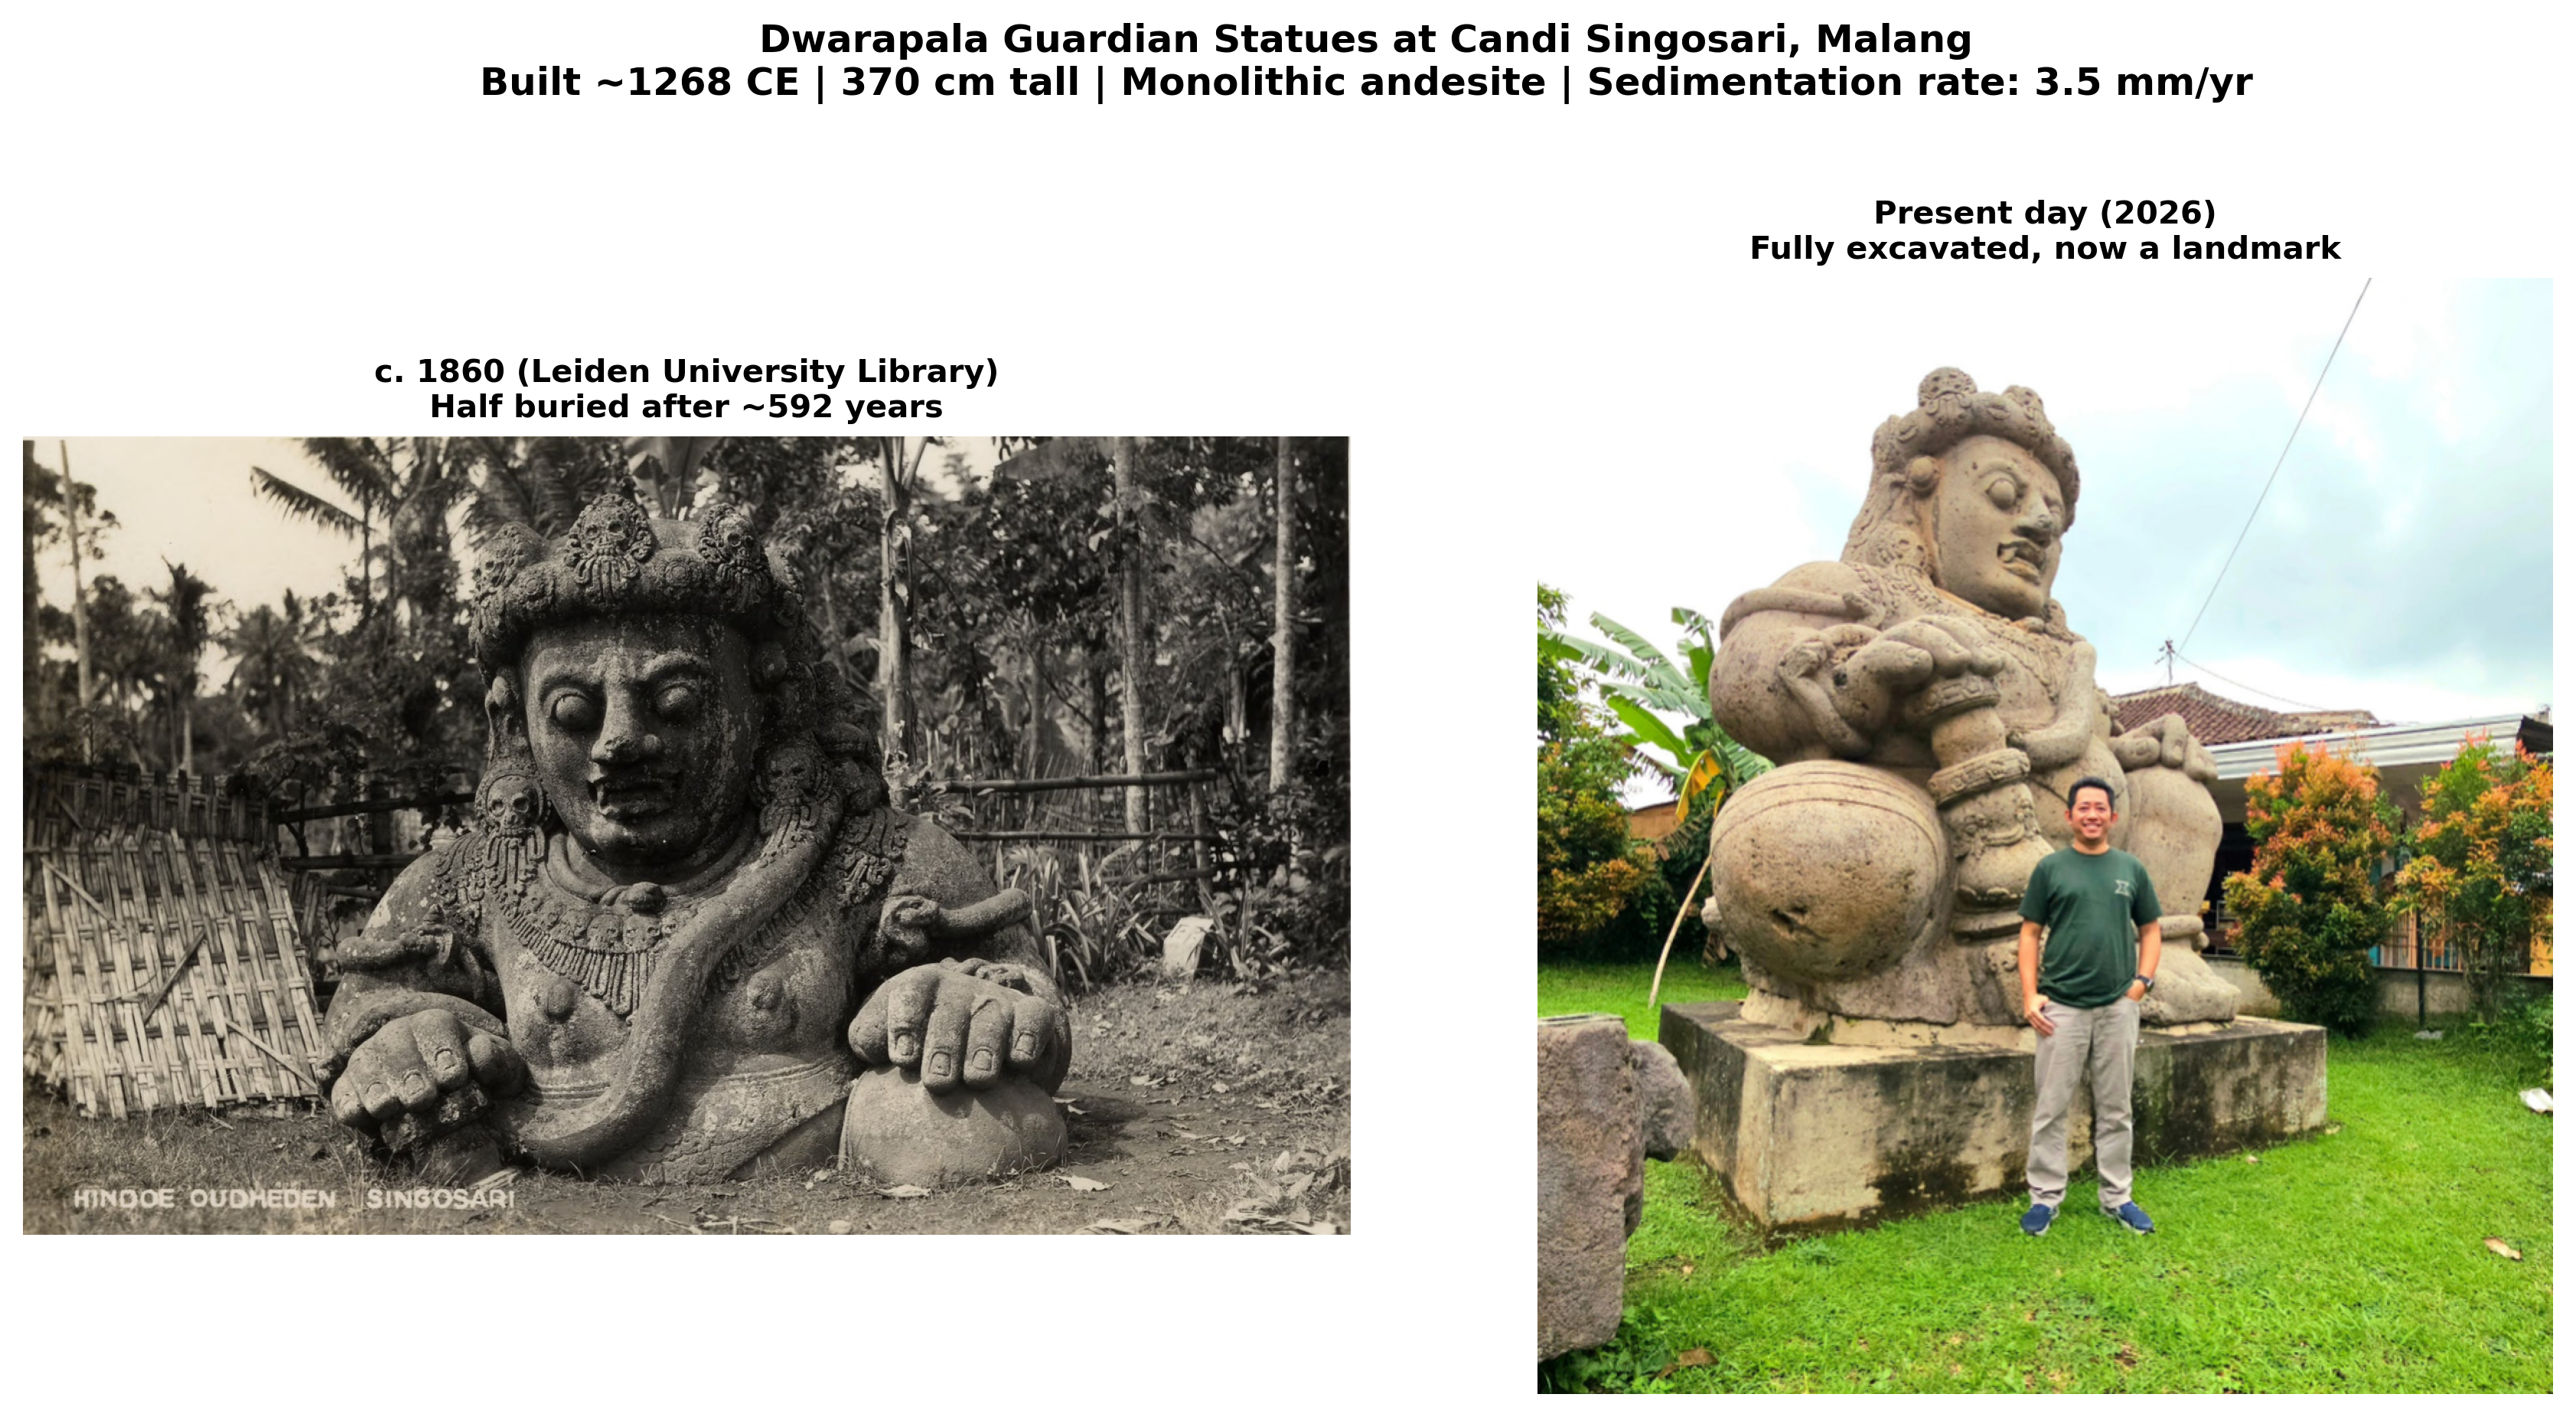
\includegraphics[width=12cm]{figures/fig0_dwarapala_comparison.png}
\caption{Dwarapala guardian statues at Candi Singosari, Malang, East Java. Left: colonial-era photograph (c.~1860) from the Leiden University Library archives, showing the statue partially buried beneath volcanic sediment---only the head, shoulders, and hands remain visible above the accumulated overburden. Right: present-day condition after excavation, revealing the full 370~cm height. The statues were constructed \textasciitilde1268~CE during the reign of Kertanegara; approximately 185~cm of volcanic overburden accumulated by their rediscovery in 1803~CE, yielding a calibrated sedimentation rate of 3.5~mm/yr (Sect.~3.2).}
\label{fig:dwarapala_photos}
\end{figure*}

Surface visibility is a recognized problem in archaeological survey \citep{wandsnider1992,french2003}, but its implications for volcanic landscapes in island Southeast Asia have been largely unexplored. Research in the region has focused on monumental stone architecture---the class of evidence most resistant to burial \citep{degroot2009}---producing an inherent circularity: stone temples are found because they protrude through sediment; their distribution is interpreted as reflecting settlement patterns; and the wooden settlements that constituted the overwhelming majority of historical habitation are overlooked entirely.

A fifth case study is worth flagging in this introduction because it addresses a concern the framework immediately raises. If the predicted depths are correct, does organic material (wood, bamboo, thatch) survive at those depths, or does tropical decay destroy it before burial completes? Candi Liangan, on the flank of Mount Sundoro in Central Java, provides a preliminary empirical answer. Discovered accidentally in 2008 during sand mining, the site is buried under 5--9~m of tephra from a catastrophic eruption sometime after the 6th century~CE \citep{abbas2016}. It preserves wooden architectural elements, carbonised rice, and other perishable material in situ. Liangan does not calibrate the rate (its burial was catastrophic, not cumulative), but it demonstrates that the burial regime of Javanese volcanoes can preserve organic architecture when the depth is reached quickly enough. The existence of Liangan is the strongest single counter-argument to the ``the organic material is simply gone'' alternative explanation of the archaeological absence.

The surface distribution of known Javanese archaeological sites is not presented in this paper as a test of the framework. The observed distribution is heavily conditioned by survivorship bias (large stone structures dominate the record) and two centuries of survey concentration in the Singosari--Majapahit heartland. Documenting that this surface record cannot distinguish low population from taphonomic erasure is itself an analytic contribution, developed in Section~4: the visible archaeological landscape is not a sample of past settlement, it is a sample of what has resisted burial and attracted archaeologists.


\section{Background}

\subsection{Java as a volcanic burial zone}

Java hosts 45 active volcanoes across approximately 129,000~km\textsuperscript{2}---a volcanic density of 0.35 per 1,000~km\textsuperscript{2}, the highest of any major Indonesian island and approximately six times that of Sumatra (0.06/1,000~km\textsuperscript{2}) \citep{vanbemmelen1949}. The average spacing between volcanic centers is approximately 54~km, meaning that no point on Java lies more than approximately 27~km from the nearest active volcano. Since tephra from VEI~3--4 eruptions can deposit measurable ash at 50--100+~km from the source \citep{newhall1982}, the entire island falls within the depositional range of at least one---and typically multiple---volcanic centers. The relevant archaeological question is therefore not whether volcanic sedimentation occurs at a given location, but how much has accumulated since a site was occupied---a function of distance from active vents, local topography, and eruption history.

East Java province alone encompasses seven major active centers: Kelud, Semeru, Arjuno-Welirang, Bromo, Lamongan, Raung, and Ijen. The Brantas River basin---which hosted the Singosari (1222--1293~CE) and Majapahit (1293--\textasciitilde1500~CE) kingdoms---sits in the depositional path of Kelud (35~km east), Arjuno-Welirang (25~km north), and Semeru (60~km southeast). Kelud alone has produced 37 confirmed eruptions since 1000~CE \citep{gvp2024,maeno2019}.

In Central Java, Mount Merapi---one of the world's most active stratovolcanoes---has buried a cluster of 9th-century Hindu-Buddhist temples to depths of 3--7~m \citep{lavigne2000,thouret2000}. These buried temples (Sambisari, Kedulan, Kimpulan) were discovered accidentally during modern construction and mining activities, not through systematic archaeological survey.

\subsection{The observable archaeological record in East Java}

Our compilation of known archaeological sites in East Java (Sect.~3.1) identified 666 unique entries, of which only 391 (59\%) have usable spatial coordinates. The dataset is dominated by stone monuments (\textit{candi}) from the Singosari and Majapahit periods (13th--15th centuries~CE) \citep{kinney2003}. Earlier periods are poorly represented: pre-10th century sites constitute less than 5\% of the geocoded total.

This temporal distribution reflects two complementary pressures. Survey has historically concentrated on the Singosari-Majapahit heartland around Blitar, Malang, and Mojokerto. Simultaneously, older sites have accumulated more volcanic overburden and are therefore less likely to be exposed at the modern ground surface. The broader question of whether the pre-10th century absence reflects low population, non-monumental material culture, or taphonomic erasure is taken up in a companion synthesis (Amien, in preparation); the present paper addresses only the geophysical rate at which cumulative sedimentation proceeds.

\subsection{Volcanic taphonomy}

The volcanological literature on archaeological burial is dominated by catastrophic events: Pompeii sealed in eighteen hours, Candi Sambisari buried over roughly a thousand years. These are fundamentally different processes that produce different archaeological signatures.

Catastrophic volcanic burial---a single eruption sealing an entire settlement in hours---is well documented \citep{sigurdsson1985,doumas1983,sheets1992} and, precisely because it is dramatic, attracts sustained excavation attention. \textit{Cumulative} volcanic burial, by contrast, generates no single event to excavate. Ash arrives in centimeters per eruption, lahars rework it downslope, and every decade the ground surface is fractionally higher than the decade before. After five centuries, a surface that was once at ground level lies two meters underground. After fifteen centuries, it may lie at six meters depth. No emergency response is triggered; no excavation follows. The site becomes, gradually and completely, invisible to surface survey.

\subsection{A note on comparative context}

Two observations from elsewhere in the archipelago inform the calibration without being part of its argument. First, the oldest conventionally recognised Indonesian polity, Kutai Martadipura (\textasciitilde400~CE) in East Kalimantan, is known from inscribed stone pillars found near the present ground surface in a region with zero active volcanoes \citep{vogel1918,coedes1968,miksic2004}. Second, three Hindu-Buddhist temples on the Merapi flank (Sambisari, Kedulan, Kimpulan) were discovered beneath 3--7~m of volcanic sediment. These observations bracket the range of outcomes the calibration needs to explain: very shallow burial where no volcanism operates, meter-scale burial where it does. Whether the volcanic/non-volcanic contrast has broader interpretive implications for Indonesian historiography is a question beyond the scope of this paper \citep[see][]{amien_synthesis_forthcoming}.


\section{Data and Methods}

\subsection{Archaeological site dataset}

We compiled a database of known archaeological sites in East Java province from three complementary sources. First, we queried the OpenStreetMap Overpass API for all features tagged with \texttt{historic=*} within the Jawa Timur administrative boundary (bounding box: 6.5--9.0\textdegree{}S, 111.0--115.0\textdegree{}E), yielding 281 geolocated features. Second, we queried the Wikidata SPARQL endpoint for entities with coordinate property P625 within the same bounding box, recovering 16 precisely located sites. Third, we scraped the Indonesian-language Wikipedia article ``Daftar candi di Indonesia'' for 369 additional entries.

To increase spatial coverage, we geocoded the 369 coordinate-less entries using the OpenStreetMap Nominatim API with progressive query refinement. Of 369 queries, 94 returned valid coordinates within the study area (25.5\% success rate). After spatial deduplication within a 100~m radius, the final dataset contains 666 unique site entries, of which 391 have usable coordinates (58.7\% geocoding rate). Within the East Java analytical bounds, 383 geocoded sites were used for spatial analysis.

It should be noted that this dataset is heavily biased toward stone monuments (\textit{candi}) that survived volcanic burial due to their monumental scale. Wooden settlements, which likely constituted the vast majority of historical habitation, are systematically absent---precisely the pattern predicted by the taphonomic bias hypothesis.

\subsection{The Dwarapala calibration}

The primary empirical anchor for the burial depth framework is the pair of Dwarapala guardian statues at Candi Singosari, Malang Regency, East Java. The statues were constructed approximately 1268~CE during the reign of Kertanegara of the Singosari Kingdom and discovered in 1803~CE by the Dutch colonial administrator Nicolaus Engelhard. Each statue stands 370~cm in seated height and weighs approximately 40 tonnes, carved from monolithic andesite. At the time of discovery, approximately half of each statue's body was below the ground surface (``\textit{separuh tubuh terpendam}''), corresponding to an estimated burial depth of approximately 185~cm accumulated over 535 years (1803 $-$ 1268 = 535 years). The resulting sedimentation rate is:

\begin{equation}
  R = \frac{185~\text{cm}}{535~\text{yr}} = 0.35~\text{cm/yr} = 3.5~\text{mm/yr}
\end{equation}

This rate is internally consistent with the documented eruption history of Gunung Kelud. The volcano erupted approximately 20 times between 1268 and 1803~CE, and documented VEI~3--4 eruptions deposit 2--20~cm of ash at the distance of Malang (\textasciitilde35~km from the vent). Twenty eruptions at an average of approximately 5~cm per event would account for approximately 100~cm of the 185~cm total burial. The remainder (\textasciitilde85~cm) is attributable to secondary remobilization (lahars, reworked tephra), contributions from the Semeru and Arjuno-Welirang volcanic systems, and non-volcanic aggradation \citep{gvp2024,maeno2019}. The rates reported here represent \textit{total landscape aggradation} in volcanic terrain, not pure primary tephra accumulation; for archaeological burial, however, the total aggradation rate is the operationally relevant metric regardless of depositional source.

The Dwarapala burial timeline from construction to present is illustrated in Fig.~\ref{fig:timeline}.

\begin{figure}[t]
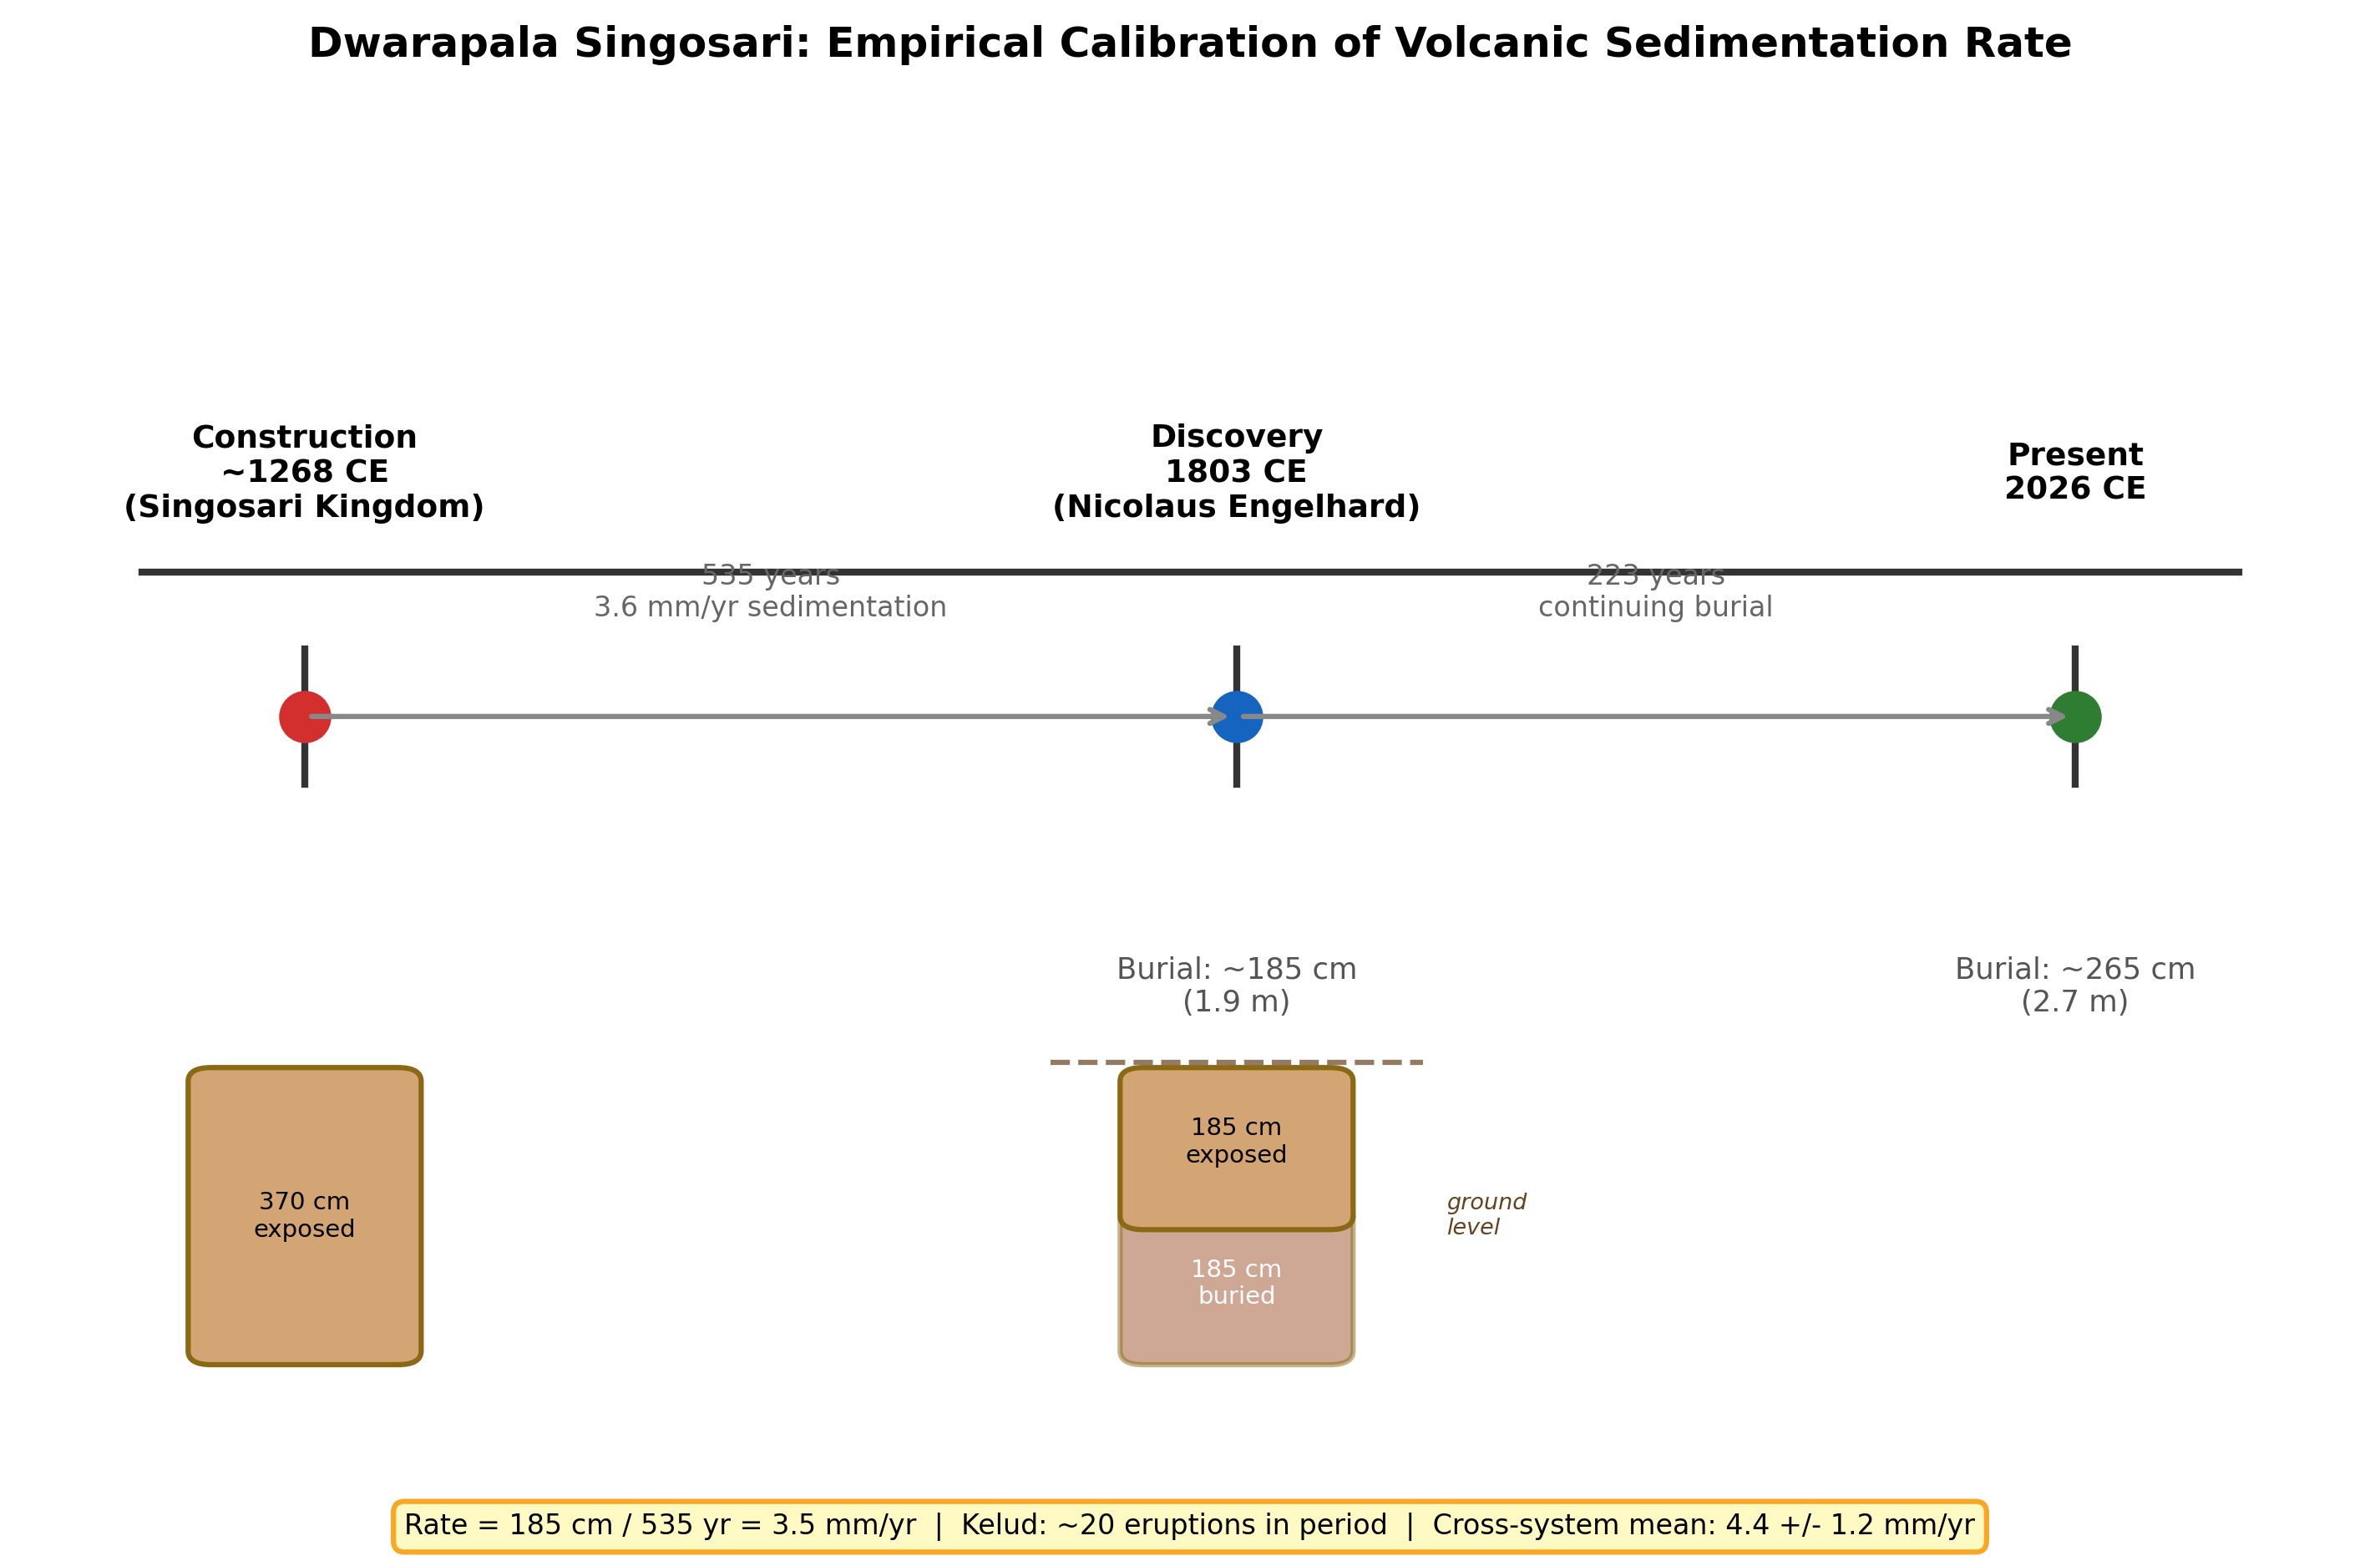
\includegraphics[width=8.3cm]{figures/fig1_dwarapala_timeline.png}
\caption{Dwarapala Singosari burial timeline. The statues were constructed \textasciitilde1268~CE at full height (370~cm) and reportedly ``half buried'' in 1803~CE according to Engelhard's colonial report, implying approximately 185~cm of volcanic overburden accumulated and a preliminary site-level rate of approximately 3.5~mm/yr. The site-level rates across four measurement anchors range 2.4--6.2~mm/yr.}
\label{fig:timeline}
\end{figure}

\subsection{Secondary calibration points}

To assess whether the Dwarapala rate is a local anomaly or representative of a Java-wide phenomenon, we compiled three additional calibration points from Central Java's Merapi volcanic system (Table~\ref{tab:calibration}).

\begin{table}[t]
\caption{Empirical calibration points for volcanic sedimentation rates at archaeological sites in Java. BPCB-Jatim and BPCB-DIY are Indonesia's regional heritage conservation agencies (\textit{Balai Pelestarian Cagar Budaya}, Ministry of Education and Culture); burial depths are from their published excavation reports. Sambisari and Kedulan depths are cited in \citet{lavigne2000} and \citet{thouret2000}.}
\label{tab:calibration}
\begin{tabular}{lcccccc}
\toprule
Site & Built (CE) & Discovered & Depth (cm) & System & Rate (mm/yr) & Source \\
\midrule
Dwarapala Singosari & \textasciitilde1268 & 1803 & \textasciitilde185 & Kelud & 3.5 & BPCB Jatim \\
Candi Sambisari & \textasciitilde835 & 1966 & 500--650 & Merapi & 4.4--5.7 & BPCB DIY \\
Candi Kedulan & \textasciitilde869 & 1993 & 600--700 & Merapi & 5.3--6.2 & BPCB DIY \\
Candi Kimpulan & \textasciitilde900 & 2009 & 270--500 & Merapi & 2.4--4.5 & \citet{putra2019} \\
\bottomrule
\end{tabular}
\end{table}

Across all four sites, the computed site-level rates span 2.4--6.2~mm/yr. Taking the midpoint of each site's range (Dwarapala: 3.5; Sambisari: 5.1; Kedulan: 5.8; Kimpulan: 3.5~mm/yr) yields an arithmetic mean across sites of approximately 4.4~mm/yr (the $\pm 1.2$ standard deviation with $n=4$ carries wide confidence bounds and is reported for description only, not as a precision estimate). The full observed range of 2.4--6.2~mm/yr is used for all subsequent projections. The order-of-magnitude agreement across two volcanic systems---Kelud in East Java and Merapi in Central Java---is consistent with the hypothesis that mm/yr-scale burial of archaeological sites occurs systematically across Java's volcanic basins (Fig.~\ref{fig:rates}), but the four-site sample, shared methodological basis, and monument-focused selection prevent this paper from establishing that consistency rigorously; see Sect.~5.6 for the constraints and Sect.~5.7 for the proposed research program.

\subsection{Literature compilation: 51 eruption--site correlations}

As a partial check on the anchor-site rates, we compiled a dataset of 51 documented eruption--archaeological site correlations from across 12 volcanic systems in Island Southeast Asia. Sources were historical and colonial-era records documenting specific volcanic events and their effects on specific known sites; 86\% of the evidence was primary (directly observed and recorded, not inferred from proximity). Of the 51 pairs, 24 include physically measured burial depths. The mean measured depth across these 24 sites is 3.41~m (median 2.50~m), order-of-magnitude consistent with the anchor-site mean rate of 4.4~mm/yr applied over a 760-year horizon (expected depth: 3.3~m). While this compilation shares no sites with the four primary anchors, it draws on the same corpus of colonial and volcanological reports and therefore inherits similar selection biases toward monumental and construction-discovered sites; it is best treated as a consistency comparison rather than as formally independent validation. The full dataset (site names, eruption events, dates, measured depths, and primary sources) is intended for supplementary release; aggregate statistics are reported here.

\begin{figure}[t]
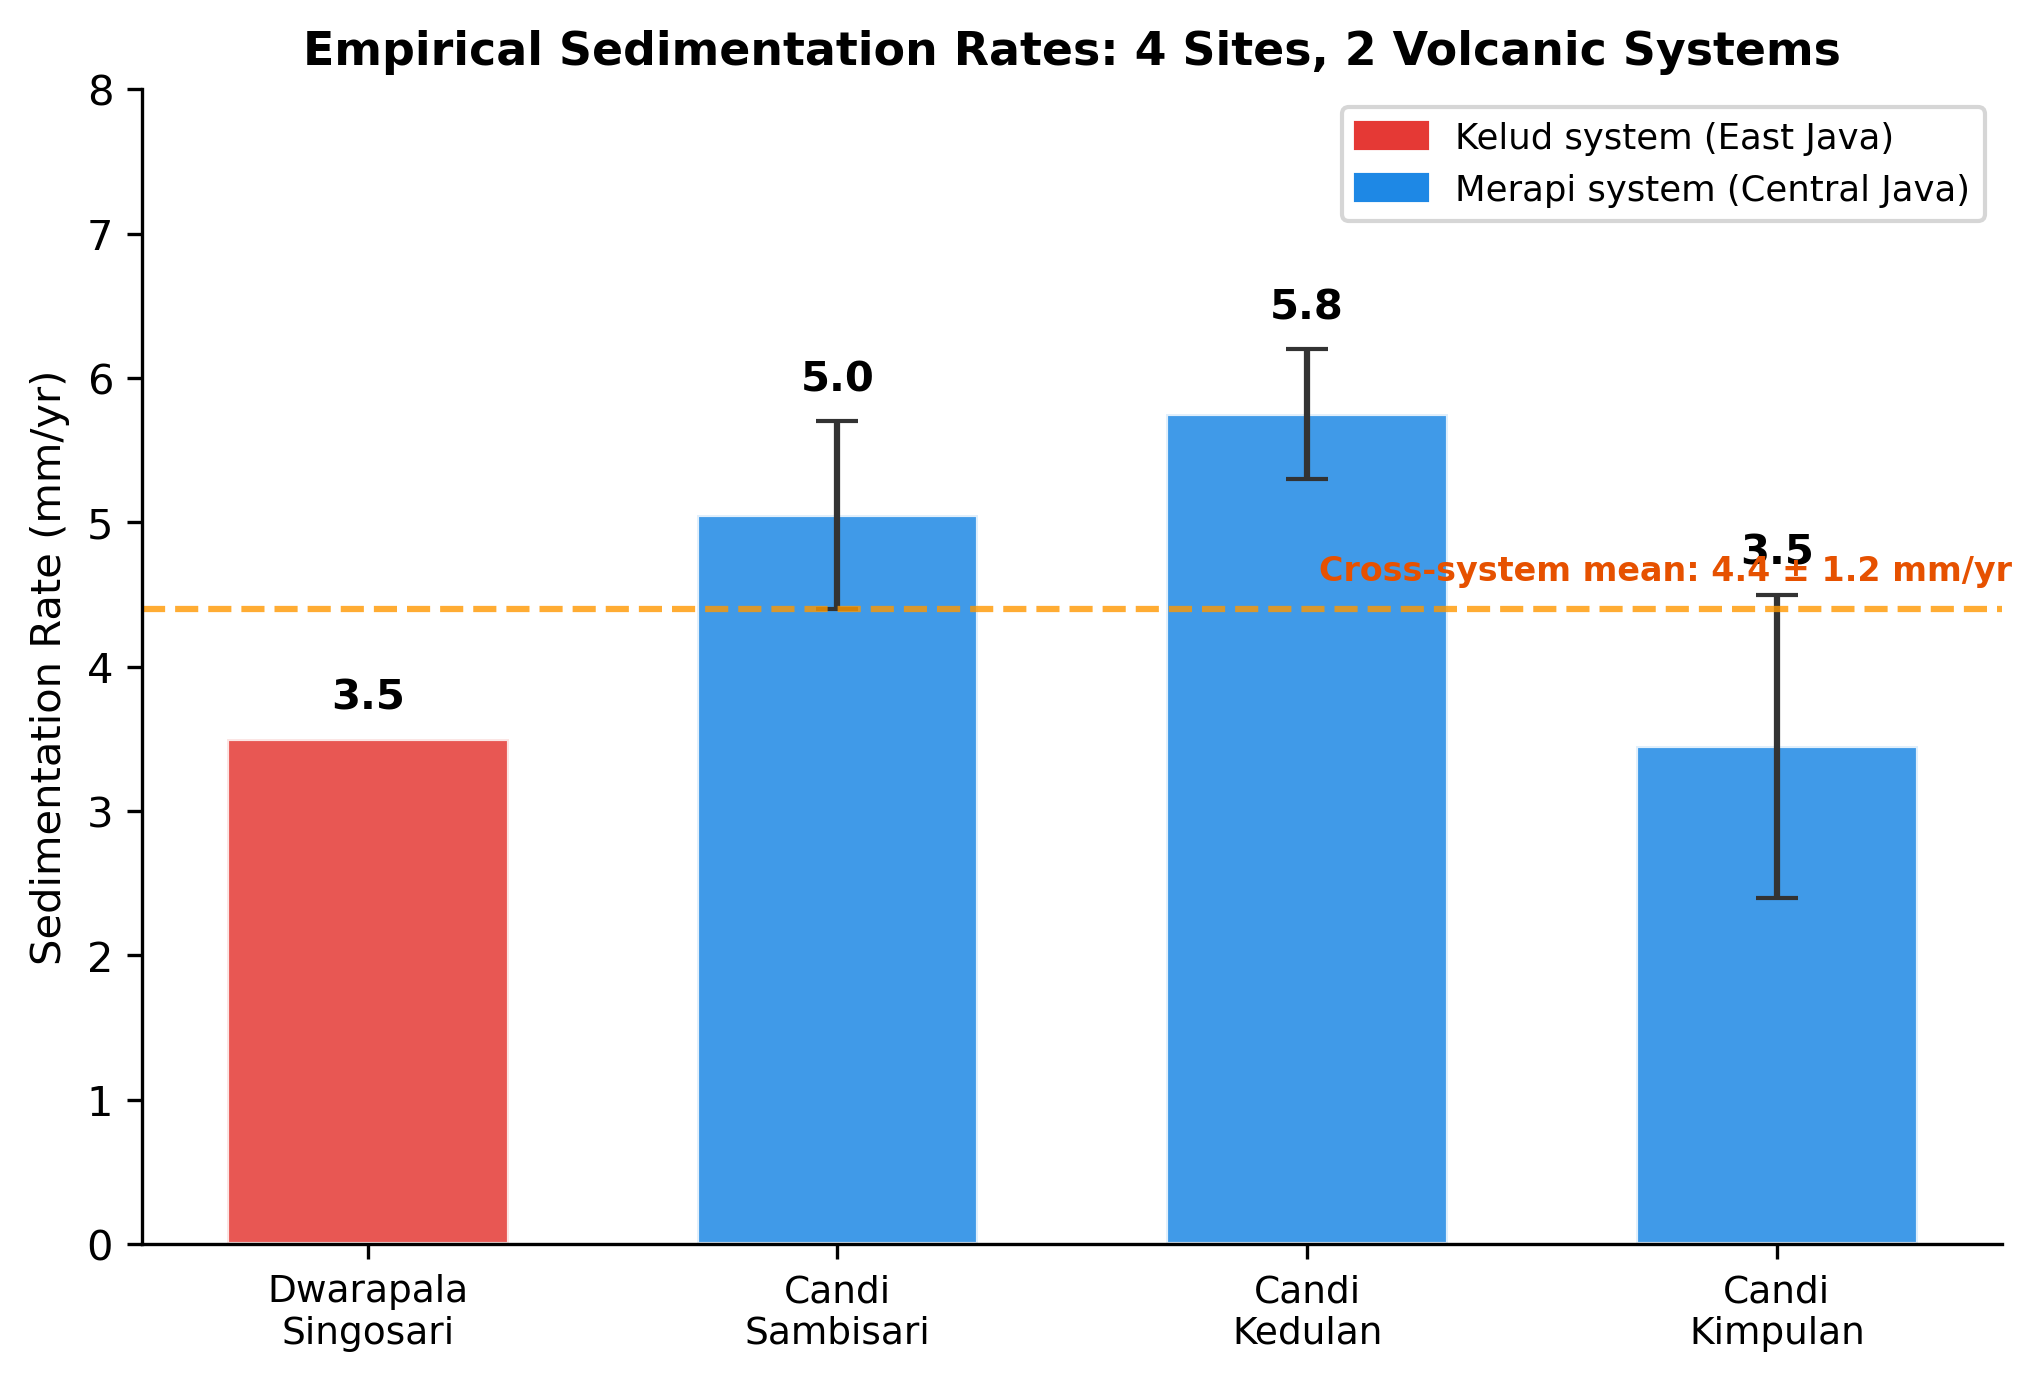
\includegraphics[width=8.3cm]{figures/fig3_calibration_rates.png}
\caption{Preliminary site-level sedimentation rates from four archaeological measurement anchors across two volcanic systems. Error bars show the range from reported depth uncertainty. Site-level rates fall within a single order of magnitude (2.4--6.2~mm/yr); the arithmetic mean across sites is approximately 4.4~mm/yr, but with $n=4$ and shared methodological basis this is not a validated cross-regional calibration.}
\label{fig:rates}
\end{figure}

\subsection{Burial depth projection model}

Using the empirically derived rate range, we estimate expected overburden depth by era according to the linear model:

\begin{equation}
  D(\text{era}) = R \times (T_{\text{present}} - T_{\text{era}})
\end{equation}

\noindent where $R$ ranges from 2.4 to 6.2~mm/yr and $T_{\text{present}} = 2026$~CE. This linear model is a first-order approximation; actual deposition is episodic, with eruption clusters interspersed by quiescent periods and subject to compaction. The wide rate range (2.4--6.2~mm/yr) partially captures this variability. Results are presented in Fig.~\ref{fig:depth}.

\begin{figure*}[t]
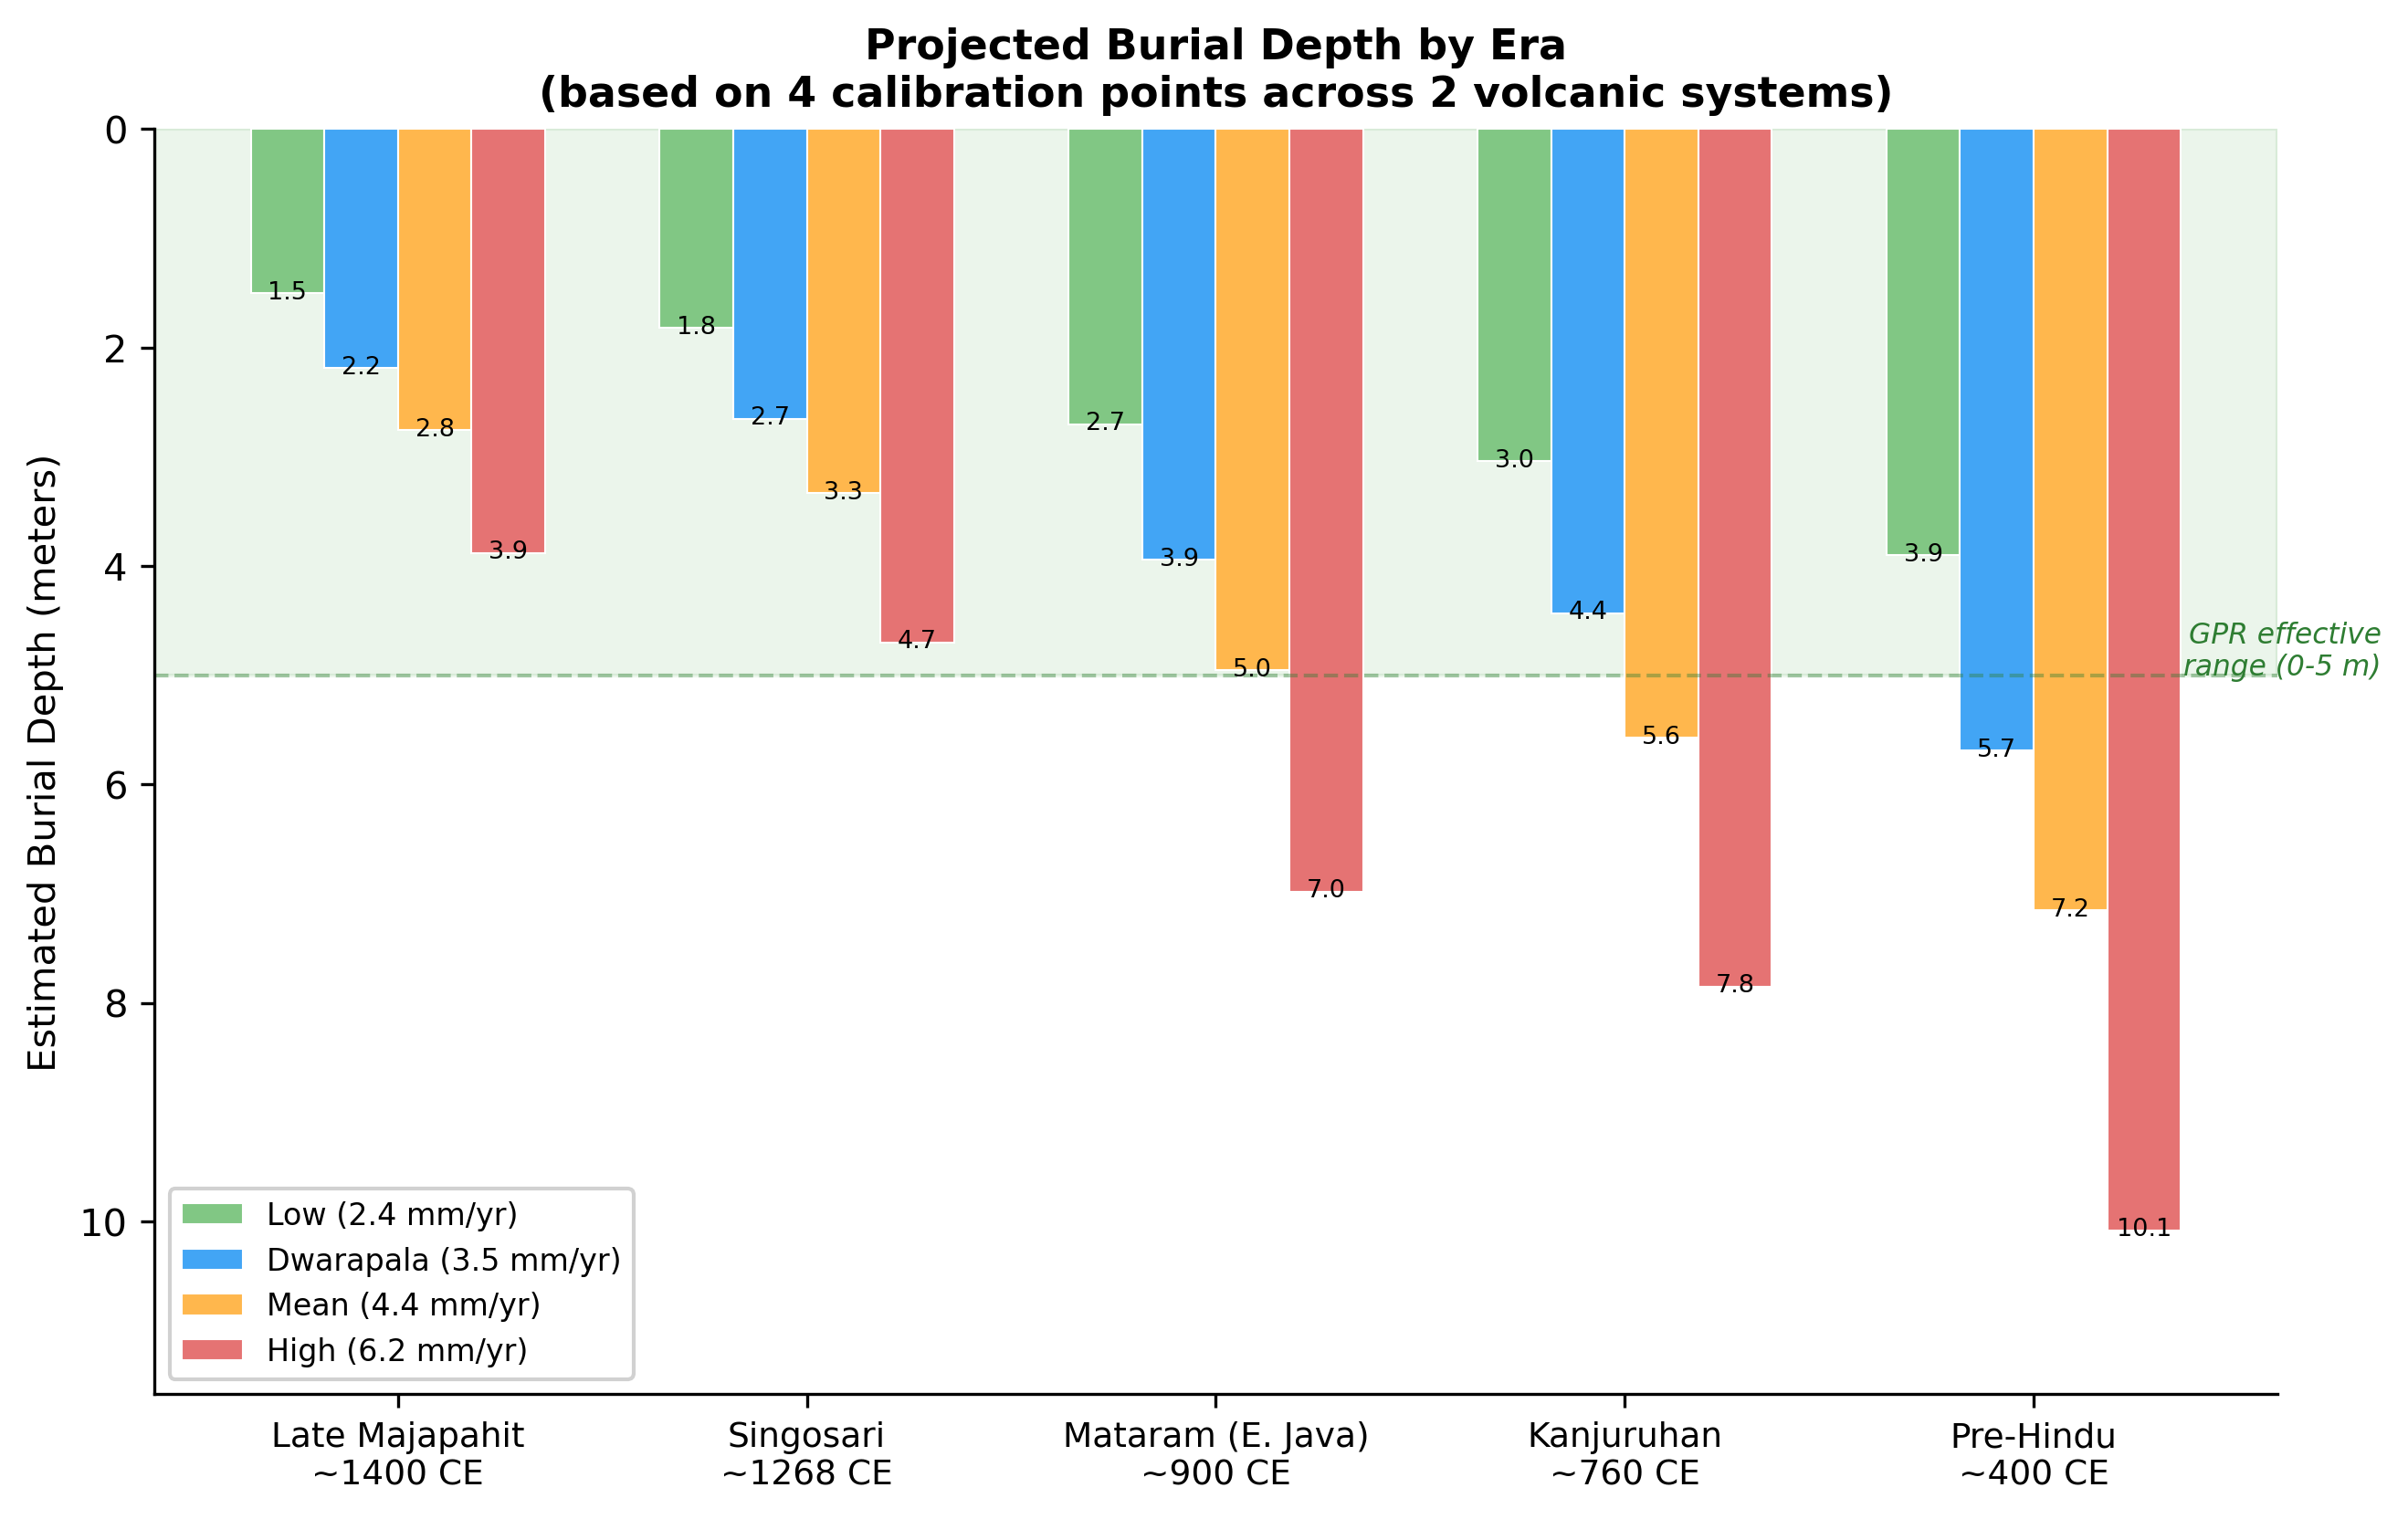
\includegraphics[width=12cm]{figures/fig2_burial_depth_projections.png}
\caption{Projected burial depth by historical era using four empirically-derived sedimentation rates. The green band indicates the effective range of ground-penetrating radar in volcanic sediment (0--5~m). Kanjuruhan-era and earlier remains may exceed GPR detection limits.}
\label{fig:depth}
\end{figure*}

\section{Results}

\subsection{The Dwarapala measurement anchor}

The Dwarapala sedimentation calculation yields a preliminary site-level rate of approximately 3.5~mm/year (Sect.~3.2), conditional on Engelhard's 1803 ``half buried'' observation being quantitatively accurate (this is discussed as a limitation in Sect.~5.6). The rate is internally consistent with documented Kelud eruption histories, which account for approximately 100 of the 185~cm total inferred burial through direct tephra deposition alone. The remaining 85~cm is attributable to secondary remobilization and contributions from other volcanic systems.

The Merapi-system anchor sites yield rates of 2.4--6.2~mm/yr, consistently higher than the Dwarapala rate (3.5~mm/yr) from the Kelud system. This difference is physically plausible: Merapi erupts more frequently than Kelud, and the Central Java sites are closer to their volcanic source. The four site-level rates fall within a single order of magnitude---a pattern that is suggestive but does not by itself establish ``Java-wide'' applicability. With $n=4$ and a shared methodological basis (depth divided by elapsed time at dated construction), formal calibration requires the additional measurement strategies outlined in Sect.~5.7.

\subsection{Literature-compilation comparison}

The 51-pair eruption--site correlation dataset is a literature compilation intended as a partial check against the four primary measurement anchors. Of the 51 pairs, 24 include physically measured burial depths, with a mean of 3.41~m (median 2.50~m). Applying the anchor-site mean rate of 4.4~mm/yr over 760 years (the midpoint historical horizon) predicts 3.3~m, which is consistent in order of magnitude with the literature compilation. We emphasise two caveats. First, the 51-pair dataset was compiled from the same corpus of colonial and volcanological reports that document the four anchor sites; the two lines of evidence share selection biases toward monumental and construction-discovered contexts, and therefore are not fully independent in the strict sense. Second, the full 51-pair table (site names, eruption events, dates, measured depths, and primary sources) is intended for supplementary release with this manuscript; the present discussion reports aggregate statistics only. The comparison is consistent with---but cannot by itself confirm---the anchor-site rates as representing a regional baseline rather than a monument-specific artefact.

\subsection{Burial depth projections}

Applying the full anchor-site rate range (2.4--6.2~mm/yr) as a first-order linear projection at basin locations, we estimate order-of-magnitude burial depths for successive historical eras. Late Majapahit-era surfaces (\textasciitilde1400~CE) lie at roughly 1.5--4~m; Singosari-era (\textasciitilde1268~CE) at roughly 2--5~m; Mataram-era (\textasciitilde900~CE) at roughly 3--7~m; Kanjuruhan-era (\textasciitilde760~CE) at roughly 3--8~m; and pre-Hindu (\textasciitilde400~CE) at roughly 4--10~m. These ranges are deliberately coarse. They assume linear extrapolation across an episodic process, ignore spatial heterogeneity across basins and flanks, and should be read as expected orders of magnitude rather than engineering-grade predictions. At depths exceeding approximately 5~m, sediment compaction of 10--30\% is expected to reduce realised depth relative to uncompacted projection. On ridges and hillslopes, erosion may dominate and produce net negligible or negative aggradation.

With those caveats, the implication for archaeological detectability is direct: surfaces of all pre-10th century Javanese occupation in basin contexts are projected to lie below the reach of conventional surface survey (0--1~m), and most lie at or beyond the effective range of ground-penetrating radar in volcanic sediment (2--5~m; \citealp{conyers2004,goodman2013}). Detecting such surfaces requires either deep coring, deep GPR, or fortuitous exposure via modern construction. The three deepest Hindu-Buddhist-era sites known in Central Java (Sambisari 1966, Kimpulan 2009, Liangan 2008) were all discovered incidentally rather than by systematic archaeological survey.


\section{Discussion}

\subsection{Site-level consistency within an order of magnitude}

The four measurement anchor sites yield rates that fall within a single order of magnitude (2.4--6.2~mm/yr), spanning two volcanic systems and 350~km of separation. For a process as variable as volcanic sedimentation---driven by eruption frequency, vent distance, wind direction, and local topography---this degree of site-level agreement is suggestive but does not by itself constitute a validated cross-regional calibration. At $n=4$ the arithmetic mean (approximately 4.4~mm/yr) has wide confidence bounds, and the Kelud and Merapi sites share a common methodological basis (burial depth divided by elapsed time since dated construction), so this is not fully an ``independent two-system'' comparison in the statistical sense.

The Kelud-system rate (Dwarapala, 3.5~mm/yr) is lower than the Merapi-system rates (central tendency approximately 4.8~mm/yr), which is physically reasonable given that Merapi erupts more frequently. Both systems produce the same order-of-magnitude result, suggesting---but not establishing---that cumulative volcanic burial operates at broadly comparable rates across Java's major volcanic basins. Whether this generalises requires the broader sampling strategy outlined in Sect.~5.7.

\subsection{Practical implications for fieldwork}

The burial depth projections translate directly into survey recommendations that differ significantly from standard practice in Indonesian archaeology. Ground-penetrating radar is effective to approximately 2--5~m in volcanic ash \citep{conyers2004}. Late Majapahit-era remains (projected depth 1.5--3.9~m) fall within this detectable range, but Kanjuruhan-era remains (3.0--7.9~m) approach or exceed the practical limits of GPR penetration. Areas with simultaneously high terrain suitability and deep predicted burial represent the highest-priority zones for subsurface investigation, as these are locations where settlement remains are most likely to be preserved yet most likely to remain undetected by surface methods. The pattern of accidental discoveries during modern construction---at Sambisari, Kimpulan, and Liangan---demonstrates that deeply buried sites exist, but systematic subsurface survey targeting such sites has never been conducted in Java.

\subsection{The Kutai--Liangan natural experiment}

The case studies examined here can be read as a natural experiment with two end members. Kutai Martadipura (c.~400~CE, East Kalimantan, zero active volcanoes) represents a surface outcome: monumental stone inscriptions from the 5th century remain at or near the modern ground surface, available to archaeological recovery without subsurface investigation. Liangan (c.~590~CE or later, Sundoro flank, Central Java) represents a deep-burial outcome: a settlement with intact wooden architecture and carbonised rice was buried under 5--9~m of tephra and recovered only when sand mining intersected it. Sambisari, Kedulan, and Kimpulan sit between these, at 3--7~m depths beneath Merapi-system aggradation.

These end members bracket the range of outcomes the framework must explain. The key inference is simple: regions of Island Southeast Asia that are geomorphologically equivalent except for the presence or absence of volcanism exhibit radically different archaeological surface records. Kalimantan preserves 5th-century inscriptions on the modern ground surface; volcanic Java requires accidental construction or sand-mining exposure to reveal even 9th-century temples. The contrast is not primarily a contrast in past occupation or institutional complexity---it is a contrast in burial regime. The archaeological record of volcanic Java has been sampled largely where the process has failed to proceed completely, and the apparent chronological primacy of Kutai may therefore reflect differential preservation rather than temporal priority.

\subsection{What the surface distribution of known sites cannot tell us}

A compilation of 666 reported archaeological sites in East Java, of which 391 are geocoded, shows strong clustering near active volcanoes and in the Singosari--Majapahit heartland. We have deliberately not presented this distribution as a test of the burial framework. Two sources of bias make it uninformative for that purpose. First, the compiled sites are those that survived cumulative burial---predominantly stone monuments that are large enough to protrude or to be discovered during construction---not a random sample of past settlement. Second, two centuries of Indonesian archaeology have concentrated field effort around the known historical kingdoms, producing a distribution that maps survey activity at least as much as it maps settlement history.

This is not merely a methodological caveat. It is a substantive finding in its own right: the surface archaeological record of volcanic Java cannot be used to argue for past cultural absence unless the detection horizon is first characterised. Reading the observed sparseness of pre-10th century open-air sites as evidence of low population, simple material culture, or absent state formation is a category error---it assumes the sample is informative when the sampling process has not been described. The framework this paper develops is intended in part to make that sampling process explicit.

The same surface record also contains a legitimate counter-observation that merits engagement: if cumulative burial proceeds at roughly 4~mm/yr, 13th--15th-century Majapahit-era stone remains should now be buried under approximately 2--3~m of sediment. Yet many Majapahit-era ruins in East Java---Trowulan, Penataran, Singosari itself---retain significant surface expression. Three non-exclusive possibilities reconcile this with the framework. First, rates are spatially heterogeneous at sub-basin scale; sites on elevated platforms or away from active aggradation zones experience lower burial. Second, ancient monumental architecture was commonly elevated on stone plinths or platforms (one to three metres above the contemporary ground surface), so that ``half buried'' in 1803 or ``near the surface'' in 2020 are consistent with 2--3~m of surrounding aggradation plus original plinth height. Third, where agricultural or ritual maintenance has actively cleared accumulated sediment, realised burial depths are lower than first-order projection would predict. None of these undermines the detection-horizon argument; all suggest that a validated rate model must incorporate spatial heterogeneity, plinth-height correction, and maintenance history---constraints the research program (Sect.~5.6) is designed to measure.

\subsection{What this paper does not claim}

Three further boundaries of the argument are worth stating explicitly. First, the anchor-site rates are derived from four stone monuments and may not transfer directly to open habitation sites, whose softer material matrix interacts with sediment and erosion differently. Monuments can trap sediment or alter local topography; landscape-scale rates for settlement contexts require direct non-monumental measurement (Sect.~5.6). Second, all four anchor sites lie in basin or plain settings. On ridges and hillslopes, erosion may equal or exceed deposition, producing different burial dynamics. The framework applies to basin contexts unless and until non-basin calibration is established. Third, we make no claim about site-type composition (caves versus open-air), population size, cultural complexity, or the broader interpretive question of what a buried pre-Hindu Javanese record might contain. Those questions depend on subsurface investigation that does not yet exist and on interpretive work that exceeds a geomorphological framework.

\subsection{Limitations}

The four measurement anchors, while spanning two volcanic systems and 350~km of Java, constitute a sample whose size and character impose several concrete limits on what this paper can claim. These limits are not cosmetic; they are why we frame the work as preliminary evidence and a research program rather than a validated calibration.

\textbf{Monument-to-settlement transferability.} All four anchor sites are stone monuments (Hindu-Buddhist \textit{candi}), not open habitation sites. Monuments are poor proxies for landscape-scale aggradation in principle: platform construction, foundation excavation, and the vertical mass of the structure itself can trap sediment preferentially or complicate stratigraphic interpretation of the original ground surface. The 51-pair literature compilation includes non-monumental contexts at a mean depth of 3.41~m that is order-of-magnitude consistent with the anchor-site rates, but this partial mitigation does not resolve the fundamental concern. The anchor-site rates should be read as bounds on the aggradation rate experienced by stone monuments, and any extrapolation to open habitation sites is an assumption that requires direct measurement at non-monumental contexts (Sect.~5.7).

Site-level rates also carry measurement uncertainty from imprecise construction dates and variable depth measurements across sources (e.g., Sambisari depths range from ``5~m'' to ``6.5~m'' depending on the source).

\textbf{Dwarapala as anecdotal anchor.} The Dwarapala observation---the only Kelud-system anchor---is a qualitative colonial description (``approximately half'' of each statue below ground) rather than a primary geoarchaeological measurement. The precise archival source requires confirmation against the original Engelhard report; we have relied on the consensus secondary-literature reconstruction \citep{kinney2003}. We have not carried out primary-source archival work at KITLV, the Nationaal Archief, or Leiden University Library where Engelhard's documents may reside. If the observation proves to reflect sculptural pedestal arrangement, later excavation backfill, or an approximation reported to indicate ``most of the statue,'' the implied Kelud rate requires substantial revision. The Merapi-system rates are independent of this specific point but share the monument-bias concern above. Future work (Sect.~5.7) proposes specific archival verification.

The sedimentation model is a first-order linear approximation. Actual deposition is episodic, with eruption clusters interspersed by quiescent periods. The wide rate range (2.4--6.2~mm/yr) partially captures this variability at multi-century timescales, but projections to intermediate intervals (50--200 years) should be treated with appropriate uncertainty. \citet{ferring1986} argues more generally that temporal variability in sedimentation rate rather than the mean rate is the dominant control on archaeological site visibility within a given basin; the multi-century-average framing here is a deliberate simplification, and site-scale visibility at any particular century may differ substantially from the mean-rate projection. Additionally, unconsolidated volcanic sediment compacts over time by 10--30\% at depths exceeding roughly 5~m; the depth estimates reported in Sect.~4.3 are therefore upper bounds, with realised depths likely somewhat shallower for the oldest eras.

The calibration sites are all located in basin or plain settings (Malang basin, Prambanan plain). On ridges and hillslopes, erosion may equal or exceed deposition, producing net negligible or negative aggradation. The framework's projections apply to basin contexts; slope locations require separate treatment.

Finally, rates derive from only two volcanic basins (Kelud and Merapi). Extrapolation to the rest of Java's volcanic terrain is provisional and requires additional calibration. The claim that survey history dominates the observed site distribution cannot be quantified precisely without systematic coverage maps, which do not exist for Indonesian archaeological survey.

\subsection{A research program for rigorous testing}
\label{sec:research_program}

The preliminary measurement anchors and literature comparison presented above are the starting points, not the conclusions, of a research program. Five specific studies, three of them achievable at modest cost in collaboration with Indonesian institutions already active in the region, would materially upgrade the evidence.

\textbf{(i) Primary-source archival verification at Dwarapala.} The Engelhard 1803 report, associated sketches, and any linked colonial survey documents should be located in archives at KITLV, the Nationaal Archief, and Leiden University Library Special Collections. Quantifying the original ``half buried'' observation (ideally with measured dimensions rather than qualitative description) would either validate or falsify the Kelud-system anchor.

\textbf{(ii) Optically Stimulated Luminescence (OSL) dating of soil profiles in non-monumental contexts.} Dated soil profiles in the Malang basin and Prambanan plain, collected from settlement-candidate locations rather than adjacent to \textit{candi} foundations, would provide landscape-scale aggradation rates directly applicable to habitation contexts. OSL is well-suited to volcanic sediments where organic preservation is poor; modest cost (\textasciitilde USD 200--500 per sample) means a 20--30 sample programme across two basins is feasible at a single-grant scale.

\textbf{(iii) Tephrochronology in sediment cores away from monuments.} Dated tephra layers in soil cores provide independent chronological anchors and a direct record of cumulative deposition. Merapi and Kelud both have well-constrained Holocene tephra records; cores targeting habitation-candidate basins would yield rates that test the monument-derived anchors.

\textbf{(iv) Targeted coring and GPR at settlement-candidate sites.} Coring at locations identified by independent settlement suitability modelling \citep[see][]{amien_synthesis_forthcoming} would directly test whether archaeological material survives at the depths projected from the anchor rates. A negative result at a statistically adequate sample (e.g., 20 locations, each reaching the projected pre-400~CE depth) would be material evidence against the detection-horizon interpretation.

\textbf{(v) Expanded and transparent 51-pair dataset.} Full publication of site names, eruption events, dates, measured depths, primary sources, and methodology for the 51-pair compilation as supplementary material would allow other researchers to interrogate selection biases and contribute additional observations. This is a modest-effort deliverable that should accompany an updated version of this paper.

Taken together, these five studies would replace the ``preliminary anchors + literature compilation'' status of the present evidence with a set of rigorous, non-monumental, and methodologically diverse measurements. At that point, claims of ``Java-wide calibration'' and specific burial-depth projections for pre-400~CE contexts would be defensible in a way they are not at present.

\subsection{Future directions beyond calibration}

Once the research program above establishes validated rates, the subsequent practical contribution is in directing fieldwork. A machine learning settlement suitability model that identifies, independently of the burial depth framework, which areas of East Java would have been most attractive to pre-Hindu settlement (Amien, in preparation) can be overlaid on validated rate estimates to produce a prioritised list of subsurface investigation targets---locations where evidence is most likely to exist and least likely to have been found. The buried sites at Sambisari and Kimpulan were found by accident; the framework towards which this paper points provides a basis for finding the next ones deliberately, through targeted GPR survey and deep coring programmes.


\section{Conclusions}

The Kutai--Java contrast with which this paper opened is the empirical heart of the argument. In Kalimantan---zero active volcanoes---a 5th-century stone-inscribed polity remains visible on the modern ground surface. In volcanic Java, even 9th-century monumental temples have been exposed only by accident. The asymmetry is difficult to explain without a taphonomic mechanism. Candi Liangan, recovered beneath 5--9~m of Sundoro tephra with its wooden architecture intact, supplies direct empirical evidence that such a mechanism operates and that organic material can survive beneath it when conditions permit.

The four measurement anchors examined here yield preliminary site-level aggradation rates of 2.4--6.2~mm/yr across two volcanic systems. With $n=4$ and a shared methodological basis, this is not a validated cross-regional calibration, and we do not present it as one. It is an order-of-magnitude consistency check that motivates---rather than closes---the question of a Java-wide burial regime. The Dwarapala anchor in particular depends on a qualitative colonial observation whose primary-source verification remains outstanding.

Projected to pre-10th century centuries, these rates imply that early-historical and pre-Hindu surfaces in basin contexts now lie at depths of several meters to roughly ten meters---below the reach of conventional surface survey and at or beyond the effective range of ground-penetrating radar in volcanic sediment. The surface distribution of known sites cannot test this projection. It reflects survey history and differential monument survival, not settlement geography.

The framework's value, we argue, is not that it demonstrates a buried civilisation. It is that it characterises a detection horizon. The apparent archaeological absence of pre-10th century open-air sites in volcanic Java cannot be read as evidence of cultural absence unless that horizon is first measured directly. The research program outlined in Section~5.6---OSL dating of soil profiles, tephrochronology in sediment cores, targeted coring at non-monumental settlement candidates, primary-source archival verification at Singosari, and transparent publication of the 51-pair literature compilation---specifies how that measurement could be made. These are not grand-budget projects. They are modest geoarchaeological studies achievable in collaboration with Indonesian institutions currently active in the affected basins.

We frame this paper as an invitation: to the geomorphologists, archaeologists, and institutional actors with direct access to the Merapi, Kelud, Sundoro, and Bromo-Tengger basins, and to those positioned to fund or support such work, we offer a testable hypothesis with specific methodological steps for validation. What is needed next is not more computation. It is a soil core.


\section*{Data availability}

The archaeological site dataset, DEM derivatives, and analysis scripts are available at \url{https://github.com/neimasilk/volcarch-repo} (to be made public upon acceptance). Raw DEM data from Copernicus GLO-30 are publicly available. A preprint of this manuscript is available at \url{https://doi.org/10.5281/zenodo.19081502}.


\section*{Author contributions}

Conceptualization, M.A.; methodology, M.A. and G.F.G.; software, M.A. and G.F.G.; validation, M.A.; formal analysis, M.A.; investigation, M.A.; data curation, M.A.; writing---original draft, M.A.; writing---review and editing, M.A. and G.F.G.; visualization, M.A.

\section*{Competing interests}

The authors declare no competing interests.

\section*{Acknowledgements}

The authors thank the Global Volcanism Program (Smithsonian Institution) for open eruption data, and the OpenStreetMap and Wikidata communities for structured geospatial data.

\textit{AI assistance disclosure.} This research used AI language tools (Claude, Anthropic) for three tasks: systematic screening of historical, epigraphic, and volcanological literature; iterative design and execution of computational experiments; and manuscript drafting and revision. Research design, hypothesis formation, data selection, interpretation, and all conclusions are solely the authors' intellectual contribution. The authors take full responsibility for all claims made in this paper.


\bibliographystyle{apalike}
\bibliography{references}

\end{document}
